\clearpage
\section{Пример использования фреймворка}
\subsection{Логистическая регрессия}
Логистическая регрессия это один из алгоритмов классического машинного обучения. Она представляет собой простейший классификатор точек в $N$-мерном пространстве. Для начала опишем вид бинарной логистической регрессии. 

Логистическая регрессия возвращает оценку вероятности принадлежности точки к предсказываемому классу (обозначим этот класс меткой $1$), то есть возвращает значение из интервала $(0, 1)$. В случае бинарной логистической регрессии оценкой принадлежности к иному классу можно считать значение, возвращаемое логистической регрессией, вычтенное из 1. 

Моделью логистической регрессии является вектор весов (параметров) $(w_0,w_1, \ldots, w_N)$. Параметры $w_1, \ldots, w_N$ прилежат к переменным по соответствующим размерностям $x_0, \ldots, x_{N-1}$. Параметр $w_N$ задает смещение. Логистической регрессией задается гиперплоскость в $N$-мерном пространстве вида $w_0x_0+w_1x_1+\ldots+w_{N-1}x_{N-1}+w_N=0$. Эта гиперплоскость делит пространство на две части. В зависимости от координат точка будет лежать по ту или иную сторону от разделяющей гиперплоскости, а значит принадлежать одному или другому классу. Для оценки того, насколько глубоко та или иная точка находится в толще предсказываемого класса, используется сигмоида. 

\begin{gather*}
S(x)=\frac{1}{1+e^{-x}}
\end{gather*}

\begin{figure}[h]
    \centering
    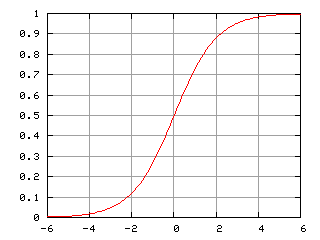
\includegraphics[width=0.6\textwidth]{Logistic-curve}
    \caption{График сигмоидальной функции.}
    \label{sigmoid_func}
\end{figure}

Сигмоида является монотонно возрастающей нелинейной функцией, определенной на области $(-\infty, +\infty)$ и принимает значения из интервала $(0, 1)$. Если точка лежит на гиперплоскости, то сигмоида примет значение равное $1/2$. В таком случае модель не может сказать о принадлежности точки тому или иному классу. Чем глубже точка лежит в толще предсказываемого класса тем ближе значение сигмоиды будет к $1$ и к $0$ в ином случае.

Для реализации многоклассовой логистической регрессии в случае $K$ классов нужно содержать $K$ векторов параметров, таких как $(w_0,w_1, \ldots, w_N)$. С помощью $i$-того вектора параметров алгоритм предсказания даст оценку принадлежности объекта к $i$-ому классу. Результирующая метка класса будет равна индексу вектора параметров, для которого предсказывающая модель дала максимальную оценку.

По своей структуре логистическая регрессия сходна с классическим искуственным нейроном с фиксированной функцией активации - сигмоидой. Логистическая регрессия может быть реализована с помощью инструментов, таких как PyTorch, Tensorflow, Keras, однако из-за популярности этого алгоритма логистическая регрессия реализована более оптимальным способом в рамках таких продуктов как scikit-learn, oneDAL, H20 и т.д.

Несмотря на простоту реализации логистической регрессии она не уступает другим алгоритмам по качеству предсказания обученной модели на многих реальных задачах. Это можно продемонстрировать на результатах, представленных в таблице \ref{ml_algs_accuracy}. Данные из таблицы были получены командой разработчиков \href{https://github.com/interpretml/interpret}{InterpretML} - библиотеки алгоритмов машинного обучения от Microsoft.

\begin{table}[h!]
\begin{center}
\caption{Сравнение качества классификации некоторых алгоритмов машинного обучения}
\label{ml_algs_accuracy}
\begin{tabular}{c|c|c|c|c}
Dataset & Domain & Logistic Regression & Random Forest & XGBoost\\
\hline
Adult Income & Finance & .907±.003 & .903±.002 & .922±.002\\
Heart Disease & Medical & .895±.030 & .890±.008 & .870±.014\\
Breast Cancer & Medical & .995±.005 & .992±.009 & .995±.006\\
Telecom Churn & Business & .804±.015 & .824±.002 & .850±.006\\
Credit Fraud & Security & .979±.002 & .950±.007 & .981±.003\\
\end{tabular}
\end{center}
\end{table}

Как можно видеть, логистическая регрессия на данных задачах показывает примерно такую же точность, как и более сложные в реализации и более требовательные к производительности компьютера алгоритмы Random Forest и XGBoost.

Оценка качества для каждого алгоритма производилась с помощью трёх случайных разбиений на тренировочную и тестовую выборки, при этом тестовая выборка составляла 25\% от общей массы наблюдений. Метрикой качества на каждом разбиении была выбрана ROC AUC.

\subsection{Граф логистической регрессии}
Вернемся к бинарной логистической регрессии. В рамках создаваемого инструмента для работы с логистической регрессией требуется создать соответствующий граф вычислений. Абстрактное представление такого графа представлено на изображении \ref{AbstractLogReg}.

\begin{figure}[h]
    \centering
    \includegraphics[width=0.3\textwidth]{AbstractLogReg}
    \caption{Абстрактное представление графа вычислений.}
    \label{AbstractLogReg}
\end{figure}

Однако описанного графа недостаточно для тренировки логистической регрессии. Для этой задачи к графу требуется добавить две дополнительные вещи:

\begin{itemize}
    \item Вершину, которая вводит в граф истинное значение класса для объекта из обучающей выборки. Эти данные необходимы для тренировки логистической регрессии, так как это один из многих алгоритмов классификации, принадлежащих к множеству алгоритмов, требующих так называемого "Обучения с учителем" (supervised learning).
    \item Функцию потерь. Эта функция показывает ошибку на конкретном объекте, и что еще важнее, позволяет вычислить антиградиент по вектору параметров модели, смещаясь в сторону которого можно уменьшить ошибку на этом объекте.
\end{itemize}

Расширенный граф, позволяющий также проводить обучение логистической регрессии, представлен на изображении \ref{LogRegWithLogLoss}.

\begin{figure}[h]
    \centering
    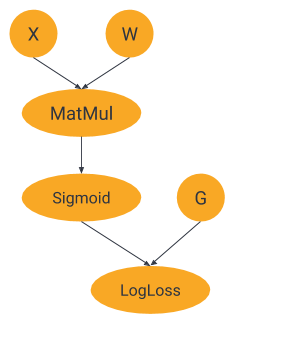
\includegraphics[width=0.4\textwidth]{LogRegWithLogLoss}
    \caption{Абстрактное представление графа вычислений, позволяющего производить обучение логистической регрессии. }
    \label{LogRegWithLogLoss}
\end{figure}

В задаче бинарной логистической регрессии используется функция $LogLoss$. Данная функция принимает на вход истинную метку класса, обозначим её за $g$. Кроме того функция принимает на вход значение, полученное из сигмоиды, которое обозначим за $a(x)$. Тогда функция $LogLoss$ будет записана в следующем виде.

\begin{gather*}
L(x, g)=g*log(a(x)) + (1-g)*log(1-a(x))
\end{gather*}

\subsection{Градиент логистической регрессии}

Для обучения модели логистической регрессии требуется вычислить градиент от функции, заданной графом. Автоматически сгенерированный градиент графа логистической регрессии, визуализированный с помощью технологии, предоставляемой \href{https://dreampuf.github.io/GraphvizOnline}{dreampuf.github.io}, изображен на рисунке \ref{GradientDot}.

\begin{sidewaysfigure}
    \centering
    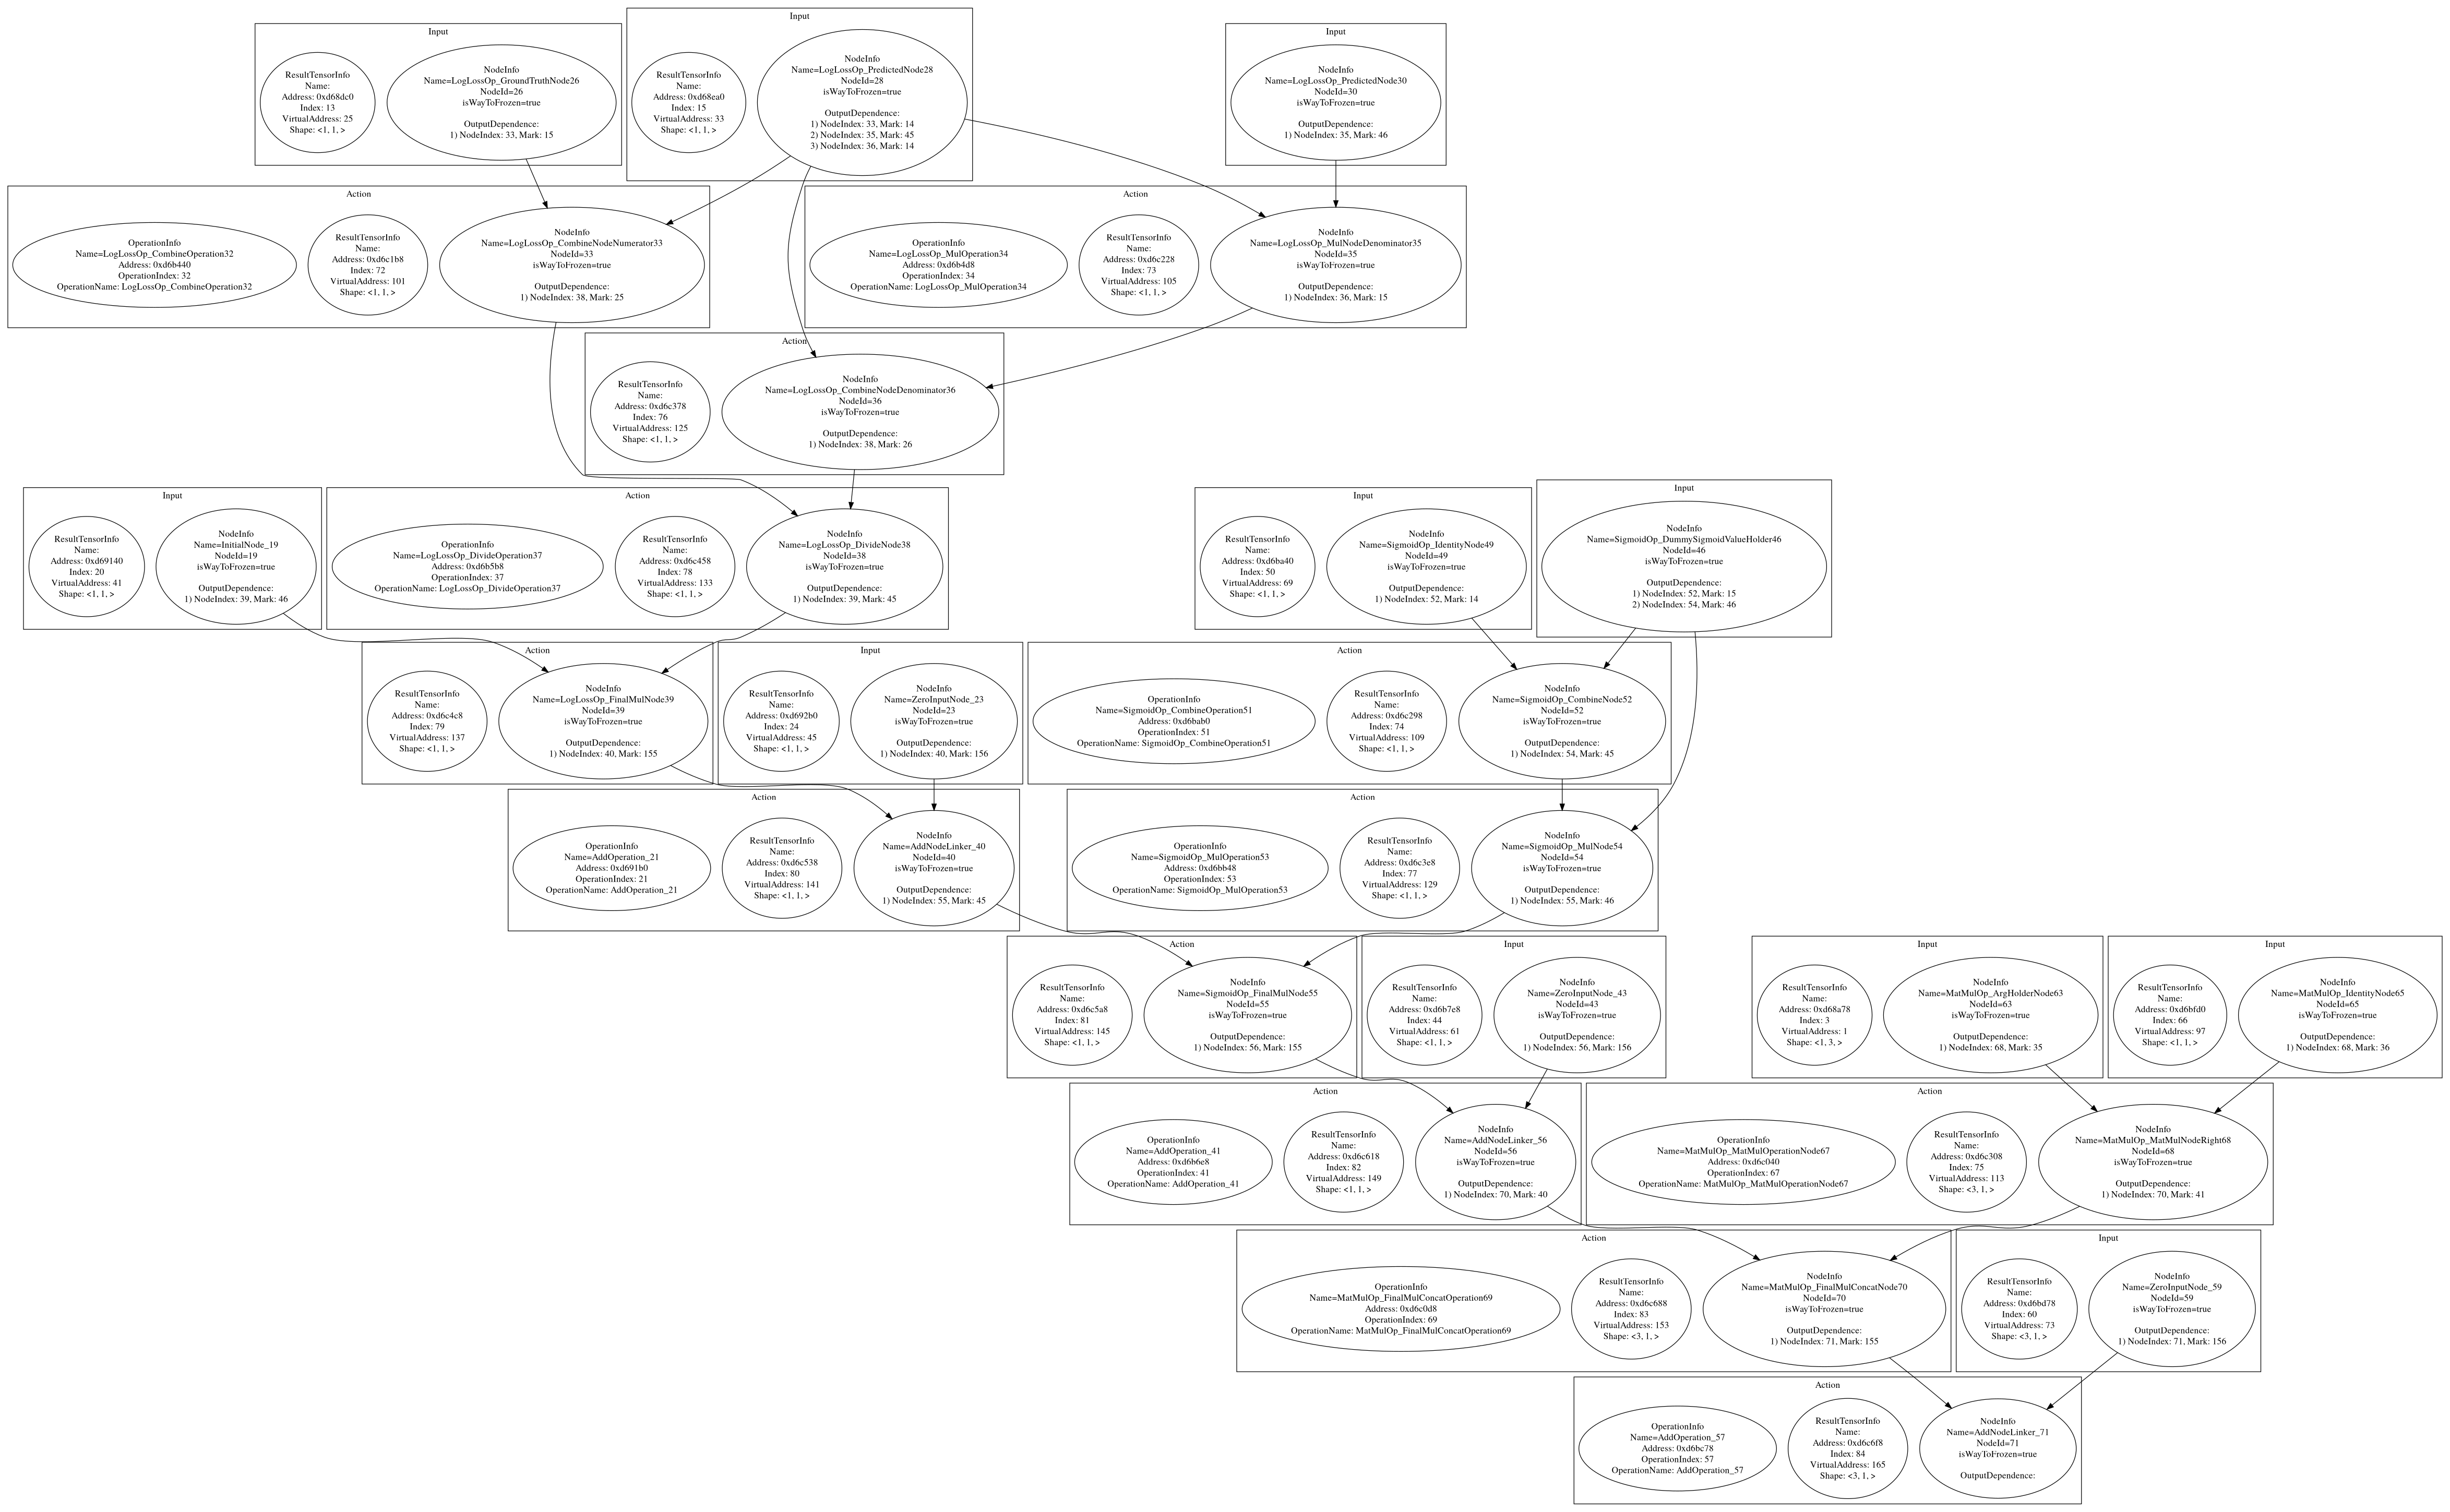
\includegraphics[width=1\textwidth]{GradientDot}
    \caption{Градиентный граф, визуализированный с помощью \href{https://dreampuf.github.io/GraphvizOnline}{dreampuf.github.io}}
    \label{GradientDot}
\end{sidewaysfigure}

% \begin{figure}[h]
%     \centering
%     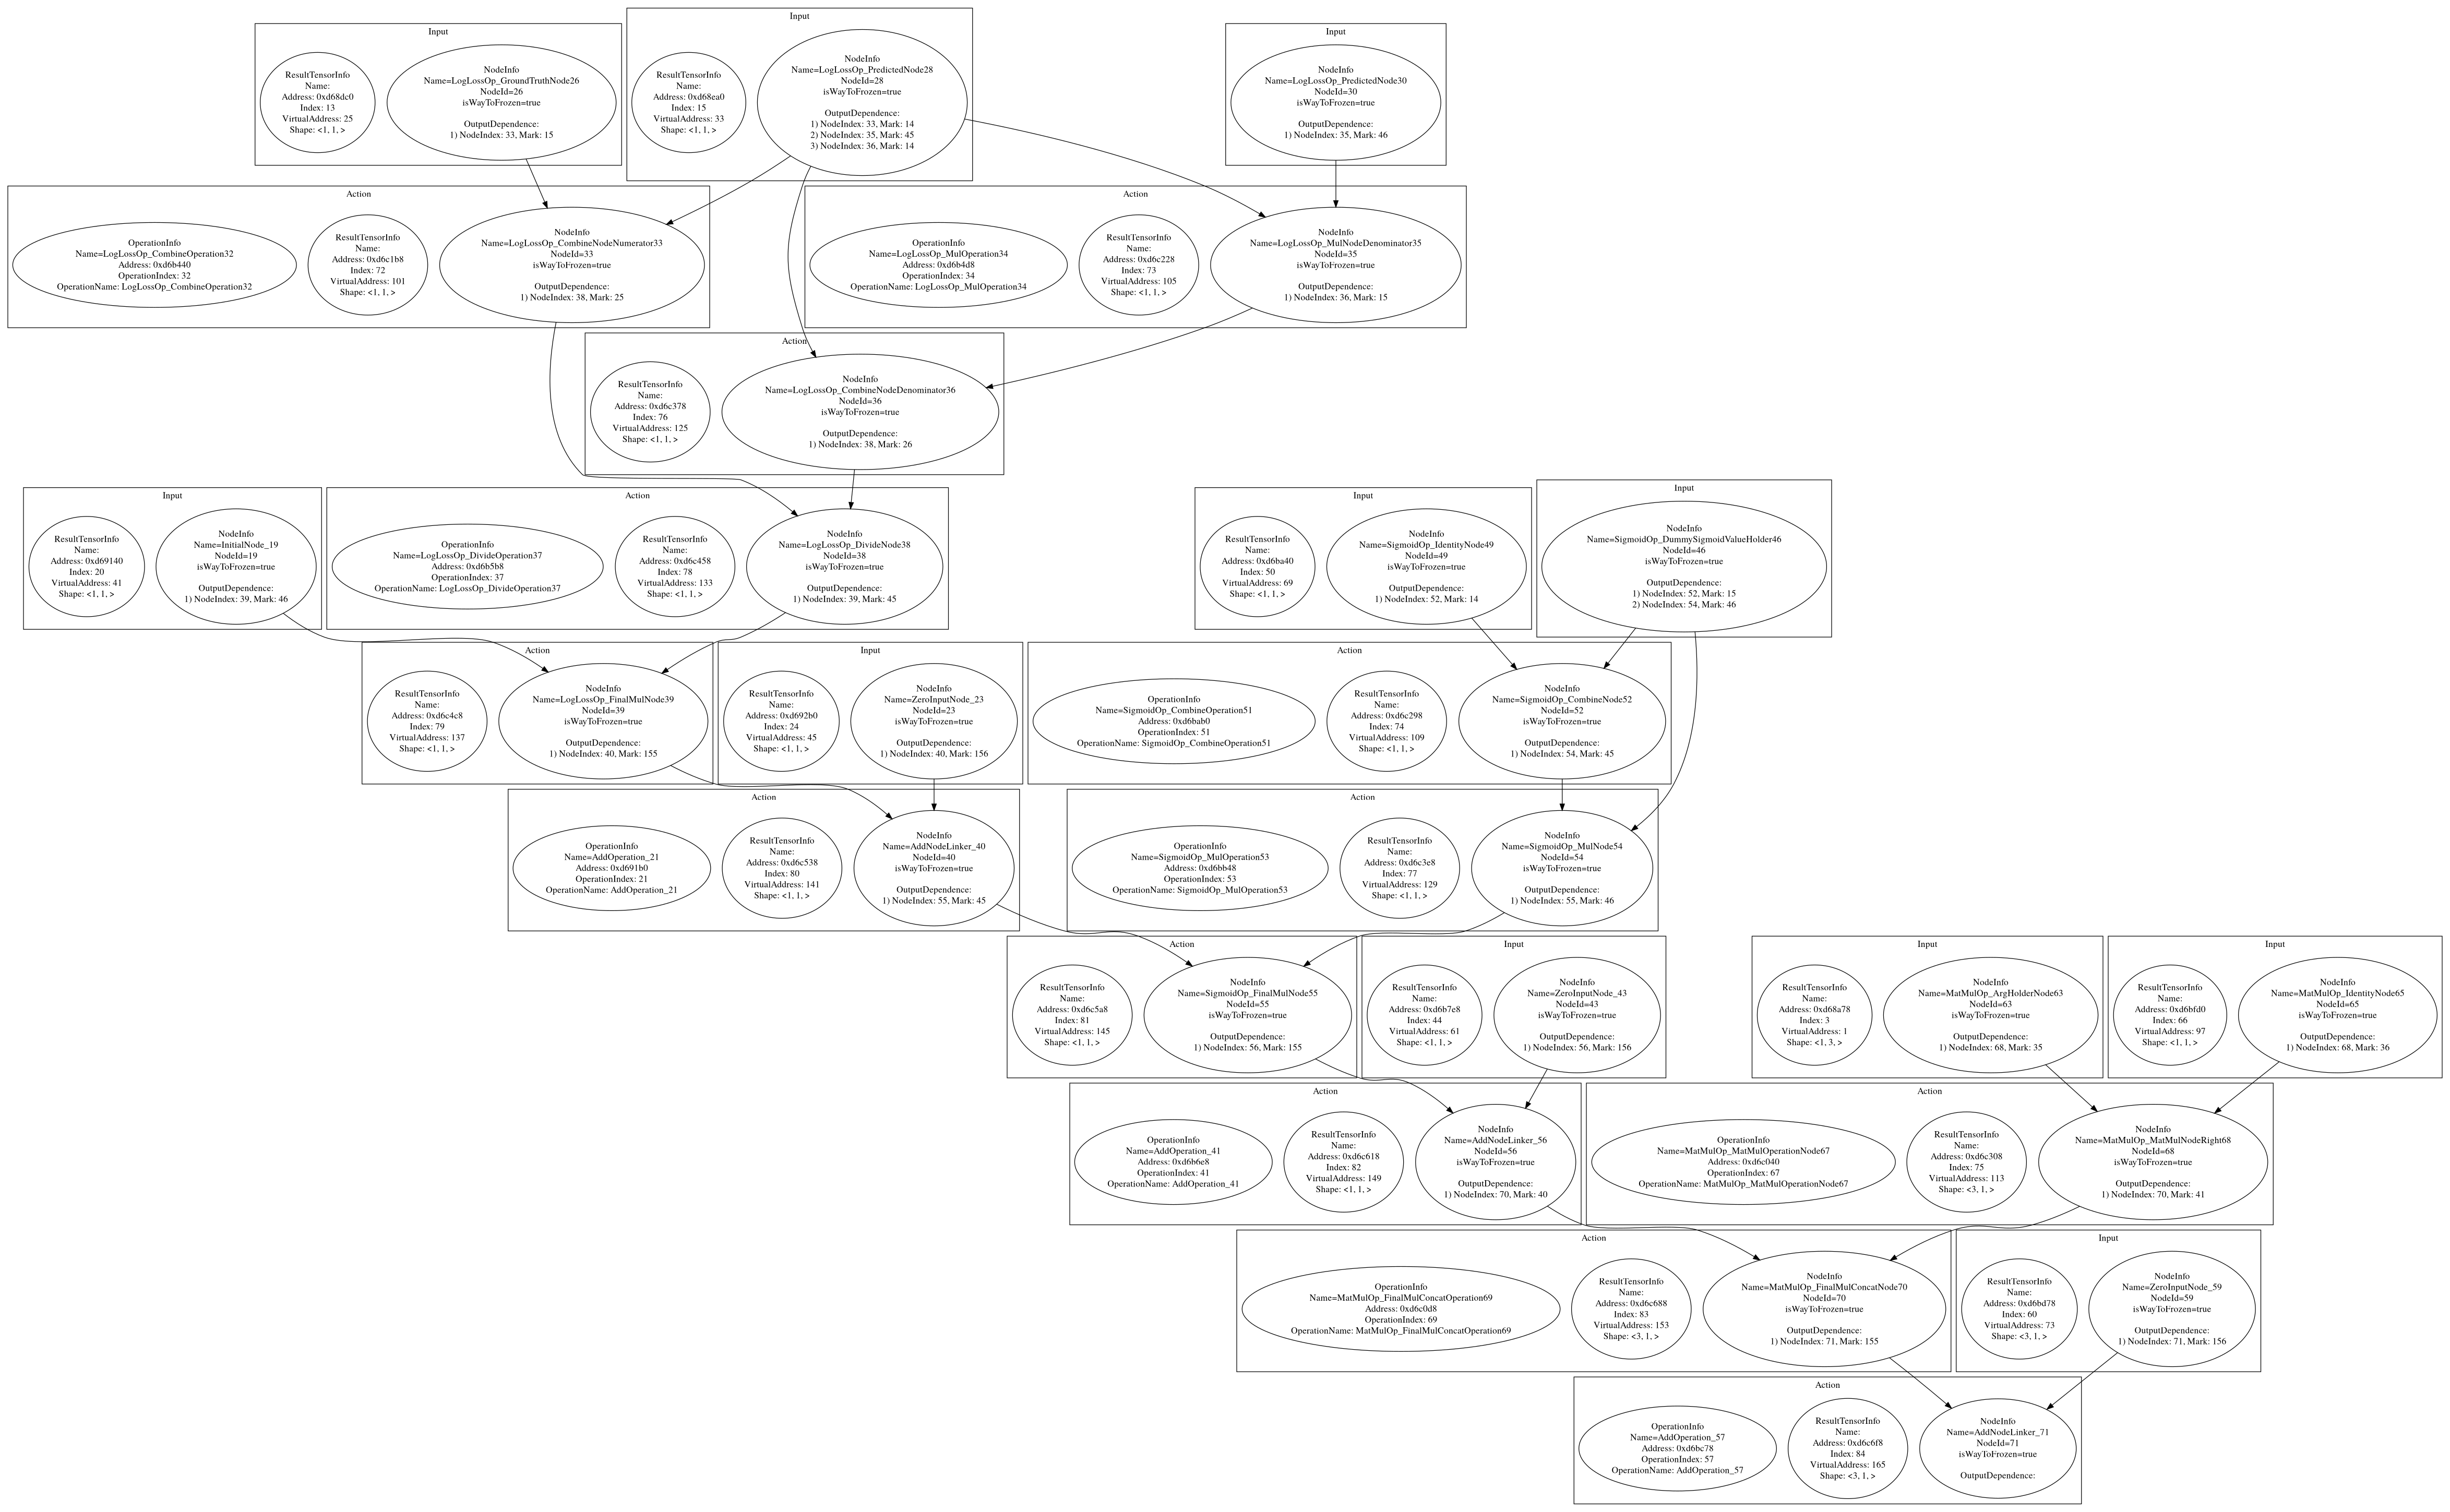
\includegraphics[width=1\textwidth]{GradientDot}
%     \caption{Градиентный граф, визуализированный с помощью \href{https://dreampuf.github.io/GraphvizOnline}{dreampuf.github.io}}
%     \label{GradientDot}
% \end{figure}

\clearpage
Для большего понимания можно представить этот граф в абстрактном виде, в котором он изображен на рисунке \ref{Grad}. На этом рисунке красным цветом выделена частная производная функции $LogLoss$ по сигмоиде, голубым - производная симгоиды по матричному умножению, и красным - матричного умножения по входу. Оранжевым цветом выделены вершины, осуществляющие умножения частных производных друг на друга для вычисления производной функции ошибки по входу графа. Также на изображении присутствуют фиктивные вершины, прибавляющие $0$. Они нужны для более простой реализации генерации градиентного графа и сгенерированный код, соответствующий им, может быть вырезан на этапе оптимизации.

\begin{figure}[h]
    \centering
    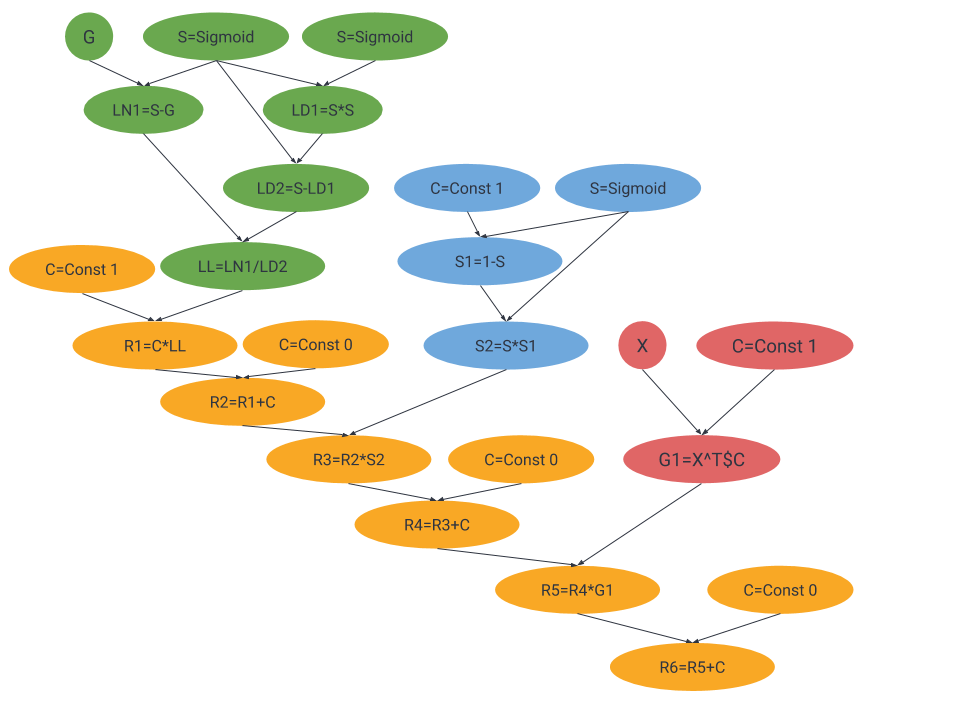
\includegraphics[width=1\textwidth]{Grad}
    \caption{Абстрактная визуализация градиентного графа}
    \label{Grad}
\end{figure}

\clearpage
Также требуется создать третий и последний связующий граф, который при вызове будет воздействовать на параметры модели значением градиента, учитывая наперед заданный коэффициент скорости обучения (learning rate). Этот граф изображен на рисунке \ref{Connector}.

\begin{figure}[h]
    \centering
    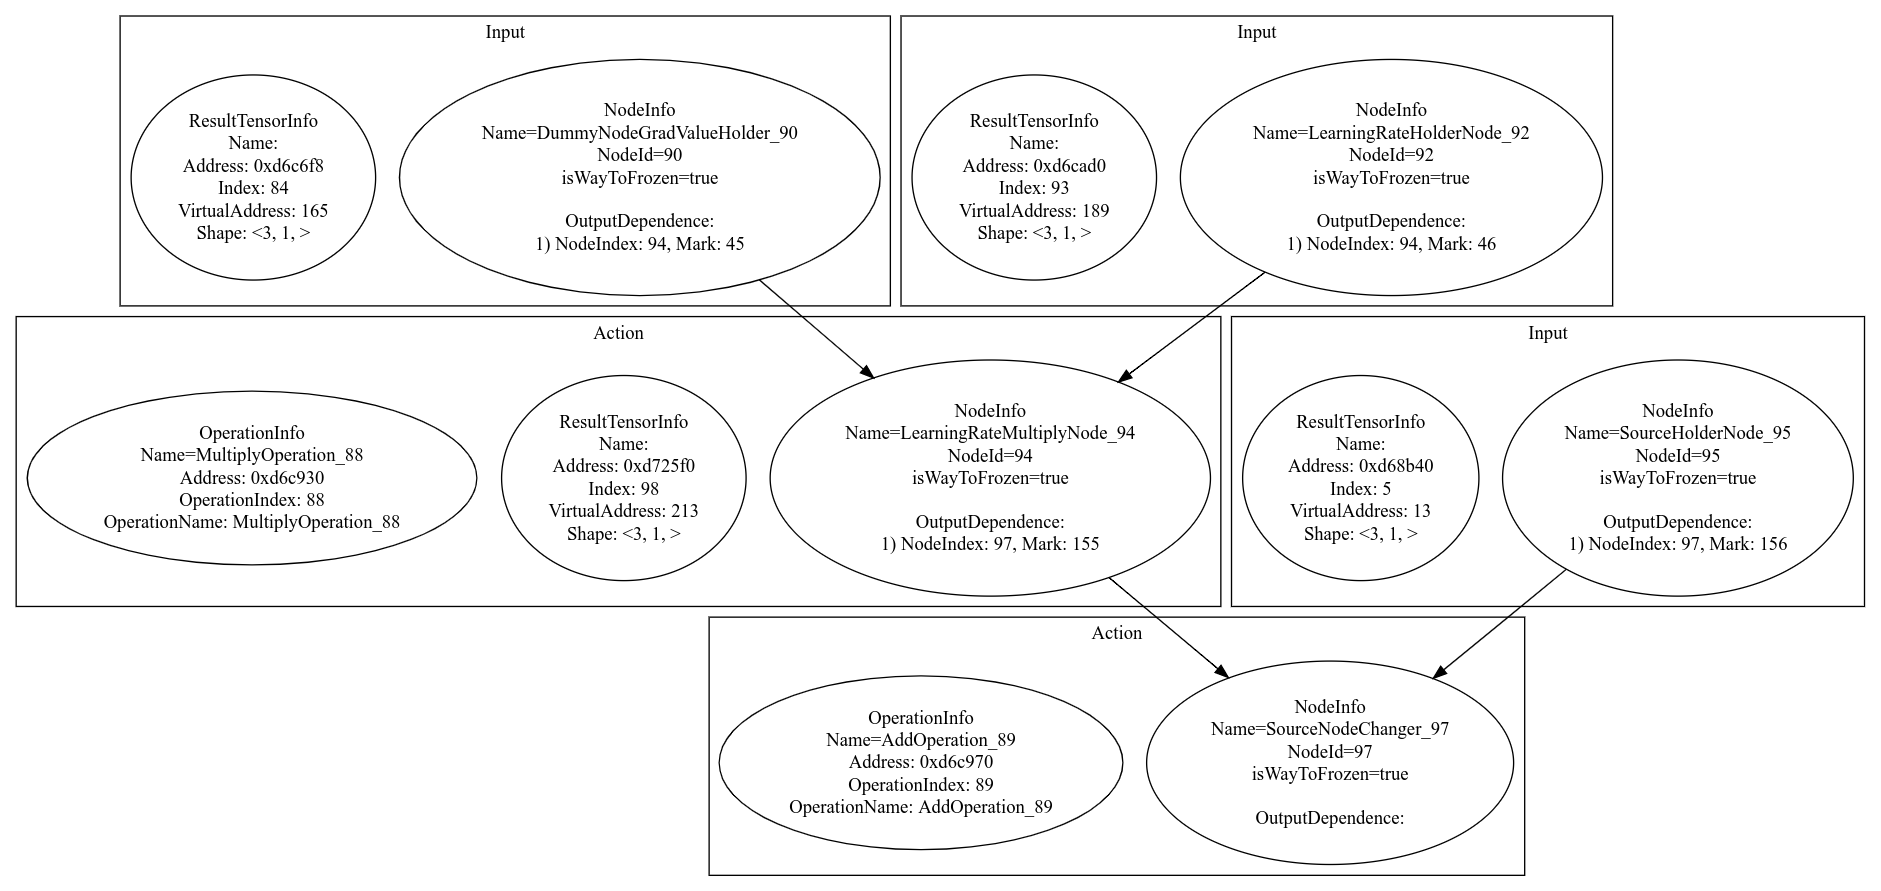
\includegraphics[width=1\textwidth]{Connector}
    \caption{Связующий граф, визуализированный с помощью \href{https://dreampuf.github.io/GraphvizOnline}{dreampuf.github.io}}
    \label{Connector}
\end{figure}

\subsection{Эксперимент с линейно разделимыми данными}
Программный код, реализующий данный эксперимент, содержится в листинге \ref{listing_log_reg} Приложения.

Для того, чтобы процесс обучения и использования модели можно было отобразить было решено рассматривать набор данных в двухмерном пространстве. В первую очередь рассмотрим работу алгоритма на линейно разделимых данных. Такие задачи в машинном обучении часто имеют не так много проблем, как задачи с линейно неразделимыми данными, особенно при применении линейных моделей.

Была сгенерирована линейно разделимая выборка, представленная на изображении \ref{data_no_intersect}.

\begin{figure}[h]
    \centering
    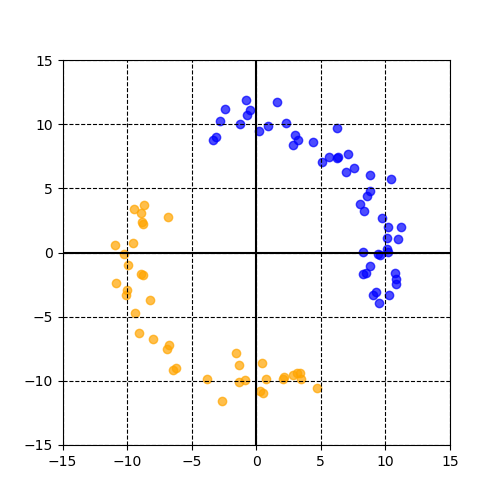
\includegraphics[width=0.6\textwidth]{data_no_intersect}
    \caption{Линейно разделимые данные}
    \label{data_no_intersect}
\end{figure}

Ниже, на рисунках \ref{training_no_intersect} и \ref{training_simple_no_intersect} представлен процесс обучения модели логистической регрессии, а также начальное и конечное положения разделяющей гиперплоскости.

\begin{figure}
\centering
\begin{minipage}{.5\textwidth}
  \centering
  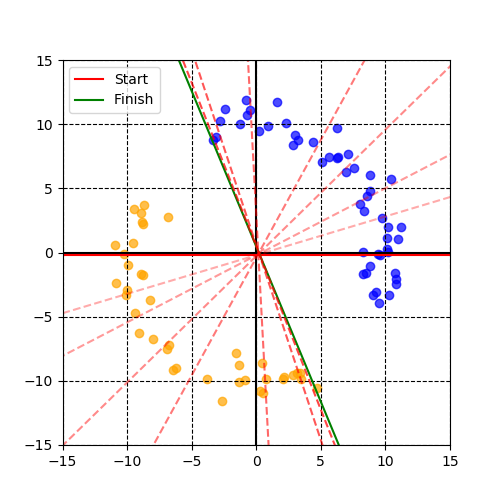
\includegraphics[width=1\linewidth]{training_no_intersect}
  \captionof{figure}{Процесс тренировки модели}
  \label{training_no_intersect}
\end{minipage}%
\begin{minipage}{.5\textwidth}
  \centering
  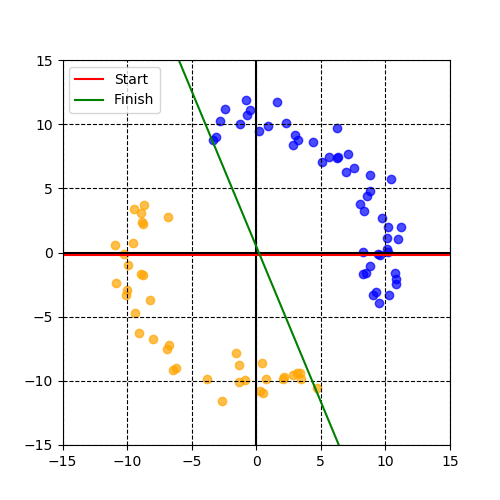
\includegraphics[width=1\linewidth]{training_simple_no_intersect}
  \captionof{figure}{Начальное и конечное состояние модели}
  \label{training_simple_no_intersect}
\end{minipage}
\end{figure}

\clearpage
Также была измерена ошибка на тестовой выборке, которая составляла половину от общей выборки. После каждой итерации была измерена суммарная ошибка с каждого элемента тестовой выборки. Результаты соответствуют ожиданиям и показаны на рисунке \ref{loss_func_no_intersect}.

\begin{figure}[h]
    \centering
    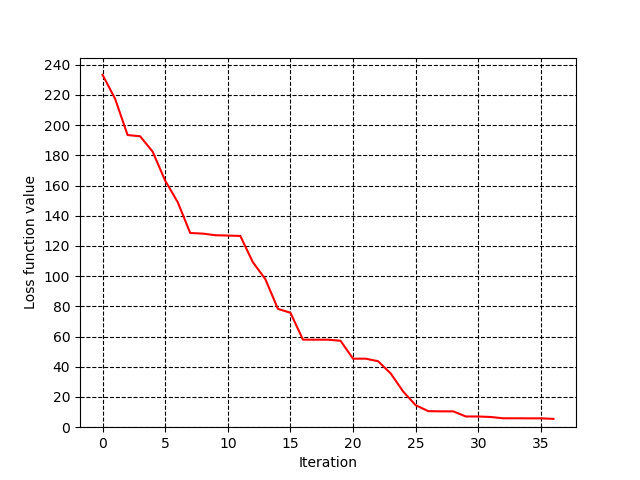
\includegraphics[width=0.6\textwidth]{loss_func_no_intersect}
    \caption{График убывания функции ошибки}
    \label{loss_func_no_intersect}
\end{figure}

На графике видно, что за 30 итераций значение функции ошибки на тестовой выборке сошлось к допустимому.

\subsection{Эксперимент с линейно неразделимыми данными}
Теперь рассмотрим вопрос обучения и тренировки логистической регрессии на линейно неразделимых данных, которые представлены на рисунке \ref{data_intersect}. Кроме того на рисунках \ref{training_intersect} и \ref{training_simple_intersect} представлен процесс обучения модели логистической регрессии, а также начальное и конечное положения разделяющей гиперплоскости. Суммарная ошибка на каждой итерации представлена на графике \ref{loss_func_intersect}.

\begin{figure}[h]
    \centering
    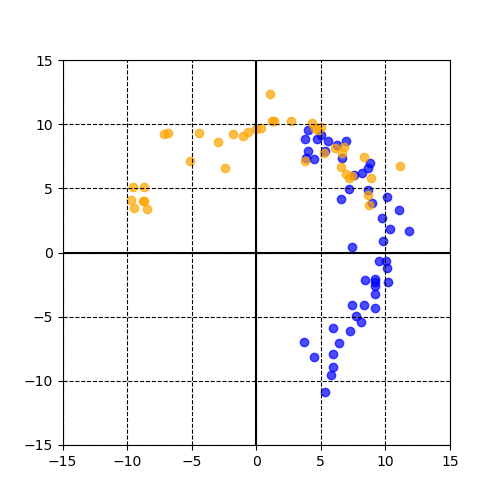
\includegraphics[width=0.6\textwidth]{data_intersect}
    \caption{Линейно неразделимые данные}
    \label{data_intersect}
\end{figure}

\begin{figure}
\centering
\begin{minipage}{.5\textwidth}
  \centering
  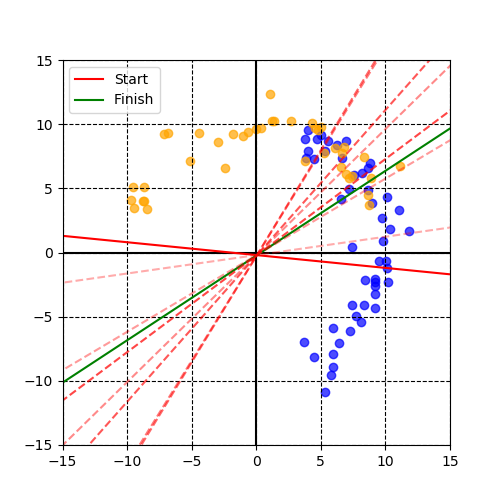
\includegraphics[width=1\linewidth]{training_intersect}
  \captionof{figure}{Процесс тренировки модели}
  \label{training_intersect}
\end{minipage}%
\begin{minipage}{.5\textwidth}
  \centering
  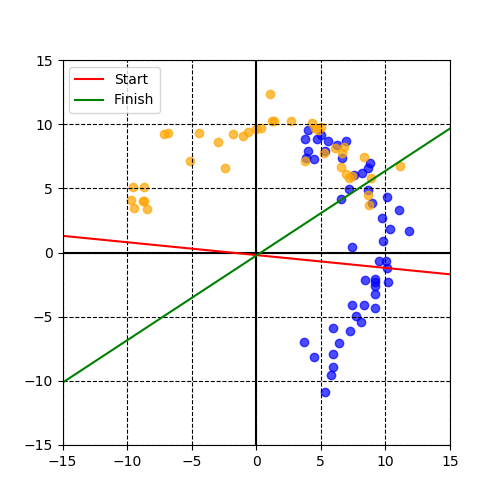
\includegraphics[width=1\linewidth]{training_simple_intersect}
  \captionof{figure}{Начальное и конечное состояние модели}
  \label{training_simple_intersect}
\end{minipage}
\end{figure}


\begin{figure}[h]
    \centering
    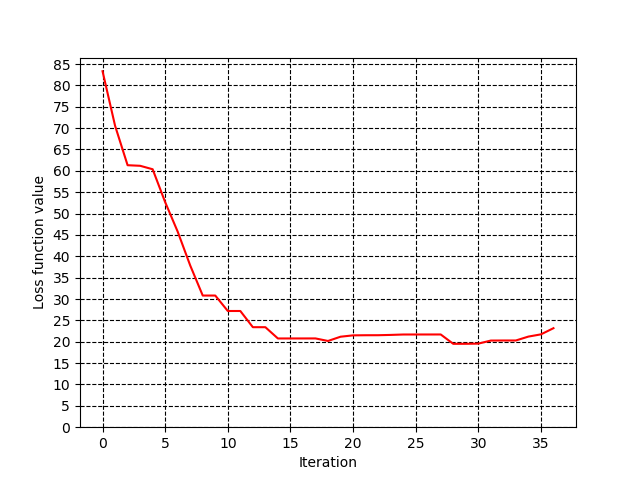
\includegraphics[width=0.6\textwidth]{loss_func_intersect}
    \caption{График убывания функции ошибки}
    \label{loss_func_intersect}
\end{figure}